\section{A reproducibility crisis}
%% THE CRISIS PART %%
\begin{frame}
\centering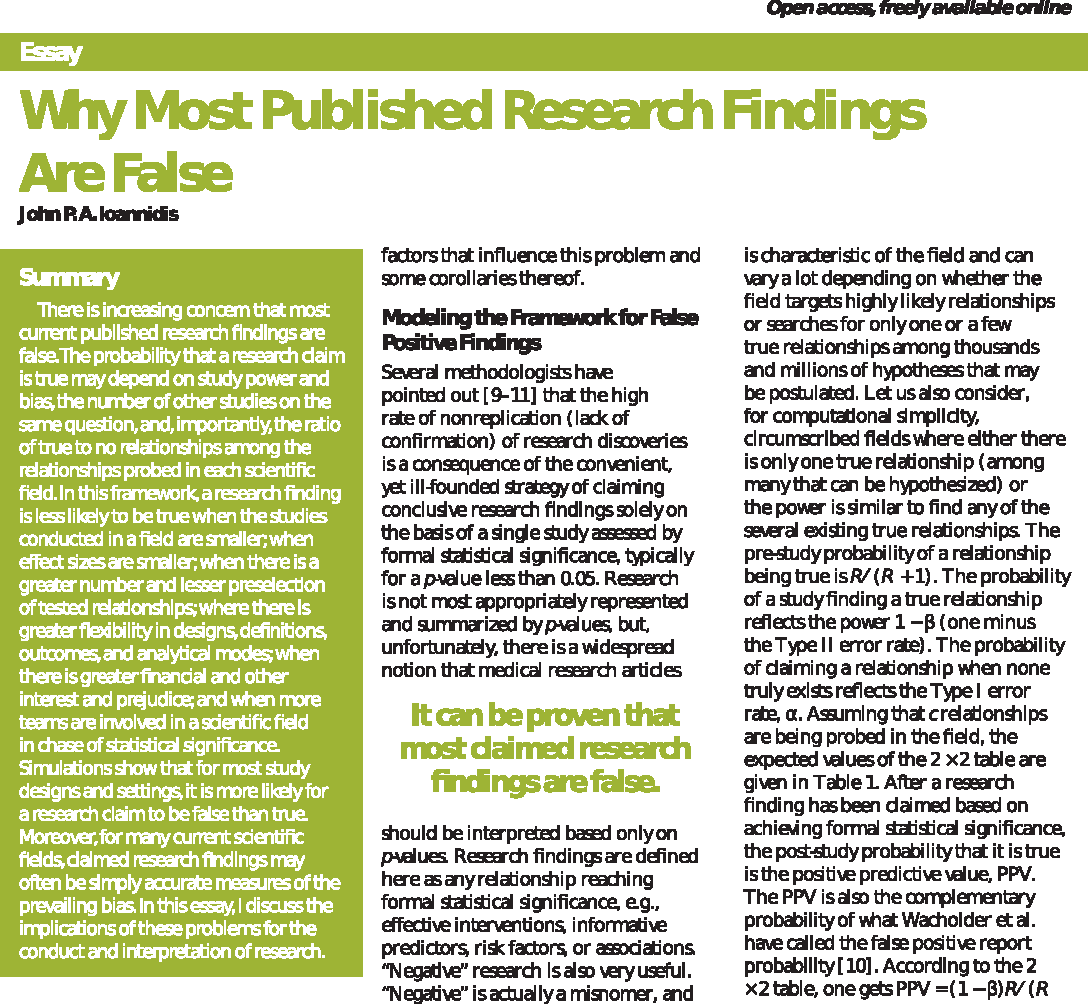
\includegraphics[scale=0.5]{/home/pierre/Seafile/ABROMICS_IFB/projet_aubi/formation_fair/fair_introduction/images/reproduce_crisis_paper.pdf}
\blfootnote{\url{https://doi.org/10.1371/journal.pmed.0020124}}
\end{frame}

\begin{frame}
\begin{block}{Crisis elements}
\begin{itemize}
\item Highlighted around 2005
\item Since 2010 more articles related to the non reproducibility
\item Medecine is one of the most impacted discipline
\end{itemize}
\end{block}
\end{frame}

%% SLIDE CRISIS FROM IFB %%

\begin{frame}
\includegraphics[page=4,scale=0.55]{/home/pierre/Seafile/ABROMICS_IFB/projet_aubi/formation_fair/fair_introduction/images/01_OS_and_FAIR_intro.pdf}
\blfootnote{\url{https://doi.org/10.1038/533452a}}
\end{frame}

\begin{frame}
\includegraphics[page=5,scale=0.55]{/home/pierre/Seafile/ABROMICS_IFB/projet_aubi/formation_fair/fair_introduction/images/01_OS_and_FAIR_intro.pdf}
\blfootnote{\url{http://reproducibility.cs.arizona.edu/v2/data/Total.png}}
\end{frame}

\begin{frame}
\includegraphics[page=6,scale=0.5]{/home/pierre/Seafile/ABROMICS_IFB/projet_aubi/formation_fair/fair_introduction/images/01_OS_and_FAIR_intro.pdf}
\blfootnote{\url{https://retractionwatch.com/the-retraction-watch-leaderboard}}
\end{frame}

\begin{frame}
\includegraphics[page=7,scale=0.55]{/home/pierre/Seafile/ABROMICS_IFB/projet_aubi/formation_fair/fair_introduction/images/01_OS_and_FAIR_intro.pdf}
\end{frame}


\section{Open science and FAIR}
%%%% FAIR history

\begin{frame}
\begin{block}{FAIR history}
\begin{itemize}
\item Born in 2016 with \textit{The FAIR Guiding Principles for scientific data management and stewardship}
\item How to build, stock, share, use and publish data
\item Make criteria to better use our data
\end{itemize}
\end{block}
\blfootnote{\url{https://doi.org/10.1038/sdata.2016.18}}
\end{frame}

\begin{frame}
\centering{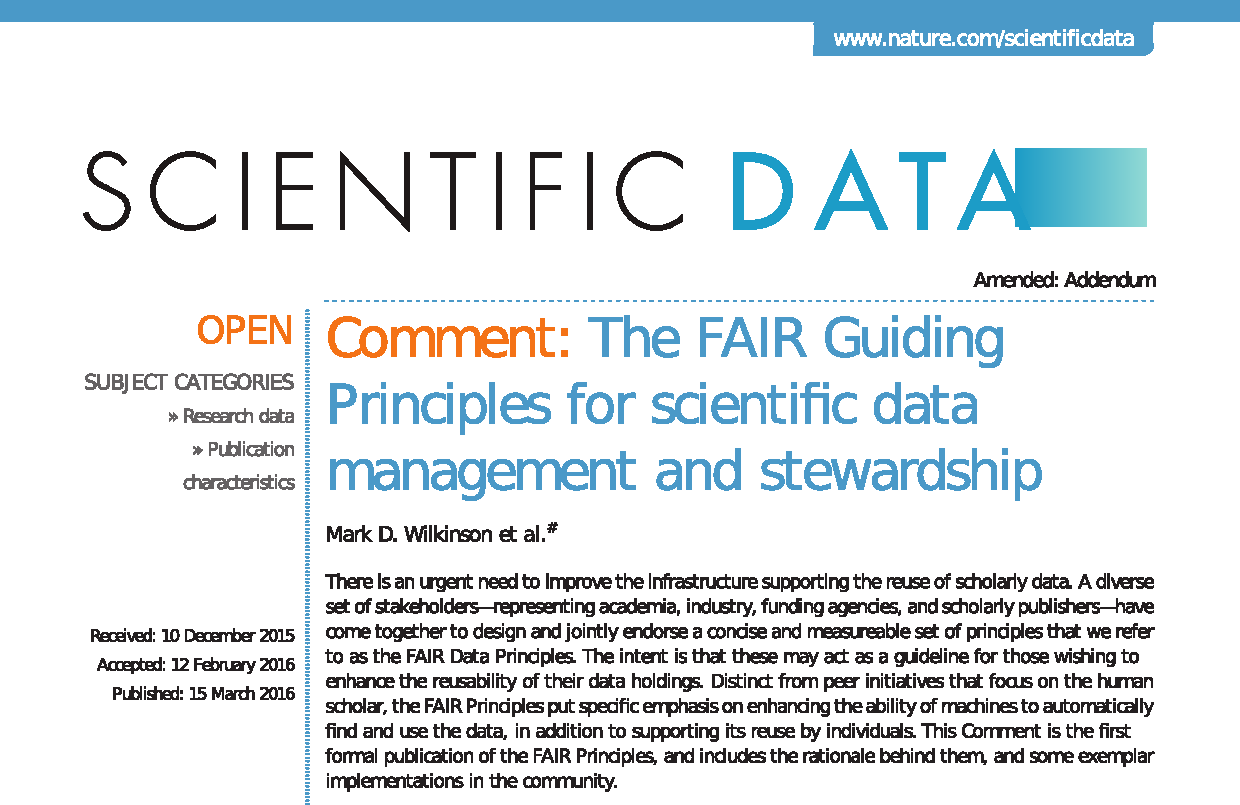
\includegraphics[scale=0.5]{/home/pierre/Seafile/ABROMICS_IFB/projet_aubi/formation_fair/fair_introduction/images/fair_paper_2016_crop.pdf}}
\blfootnote{\url{https://doi.org/10.1038/sdata.2016.18}}
\end{frame}

% FAIR for data and tools
\begin{frame}
\begin{block}{Apply FAIR TO}
\begin{itemize}
\item Your DATA
	\begin{itemize}
	\item Data lifecycle
	\item Data Management Plan (DMP)
	\item Metadata
	\item Data storage
	\end{itemize}
\end{itemize}
\end{block}
\end{frame}

% la perte des données dans le temps
\begin{frame}{Focus on the data lifecycle}
\only<1>{\centering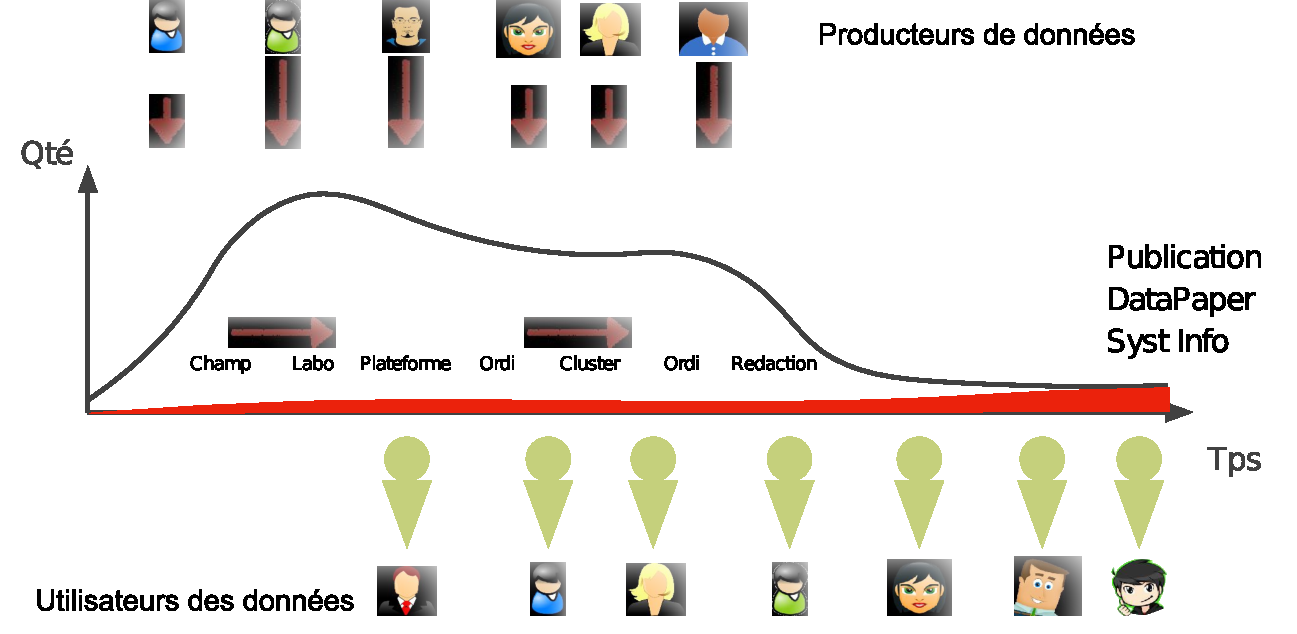
\includegraphics[scale=0.55]{/home/pierre/Seafile/ABROMICS_IFB/projet_aubi/formation_fair/fair_introduction/images/fair_data_introduction_datalife.pdf}}
\only<2>{\centering\includegraphics[page=4,scale=0.4]{/home/pierre/Seafile/ABROMICS_IFB/projet_aubi/formation_fair/fair_introduction/images/03_Organiser_son_projet_Juin_2022.pdf}}

\end{frame}

\begin{frame}{Focus on the data lifecycle}
\centering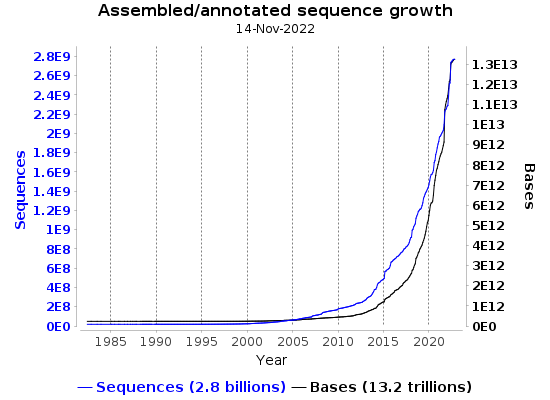
\includegraphics[scale=0.50]{/home/pierre/Seafile/ABROMICS_IFB/projet_aubi/formation_fair/fair_introduction/images/ena_embl_growth.png}
\blfootnote{\url{https://www.ebi.ac.uk/ena/browser/about/statistics}}
\end{frame}

\begin{frame}{Focus on the data exchange}
\centering\includegraphics[page=14,scale=0.45]{/home/pierre/Seafile/ABROMICS_IFB/projet_aubi/formation_fair/fair_introduction/images/03_Organiser_son_projet_Juin_2022.pdf}
\end{frame}

\begin{frame}
\centering
\includegraphics[page=1,scale=0.4]{/home/pierre/Seafile/ABROMICS_IFB/projet_aubi/formation_fair/fair_introduction/images/Cost-Benefit-analysis-for-FAIR.pdf}
\end{frame}

\begin{frame}
\begin{block}{Apply FAIR TO}
\begin{itemize}
\item Your DATA
	\begin{itemize}
	\item Data lifecycle
	\item Data Management Plan (DMP)
	\item Metadata
	\item Data storage
	\end{itemize}
\item Your scripts, environment...
	\begin{itemize}
	\item Objective of this training
	\end{itemize}
\end{itemize}
\end{block}
\end{frame}


%%%% Findable
\begin{frame}
\centering\includegraphics[page=8,scale=0.55]{/home/pierre/Seafile/ABROMICS_IFB/projet_aubi/formation_fair/fair_introduction/images/01_OS_and_FAIR_intro.pdf}
\end{frame}


\begin{frame}
\centering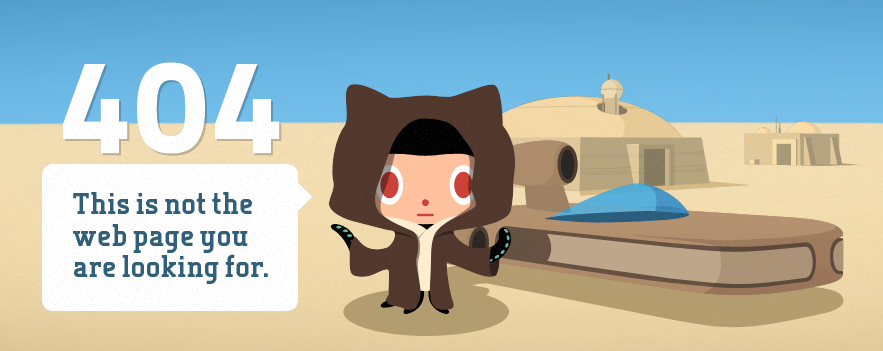
\includegraphics[scale=0.5]{/home/pierre/Seafile/ABROMICS_IFB/projet_aubi/formation_fair/fair_introduction/images/404_error.png}
\end{frame}


\begin{frame}
\begin{block}{To be Findable}
\begin{itemize}
\item (meta)data are assigned a globally unique and persistent identifier
\item data are described with rich metadata
\item metadata clearly and explicitly include the identifier of the data it describes
\item (meta)data are registered or indexed in a searchable ressource
\end{itemize}
\end{block}
\end{frame}

%%%% ACCESSIBLE
\begin{frame}
\includegraphics[page=9,scale=0.55]{/home/pierre/Seafile/ABROMICS_IFB/projet_aubi/formation_fair/fair_introduction/images/01_OS_and_FAIR_intro.pdf}
\end{frame}

\begin{frame}
\begin{block}{To be Accessible}
\begin{itemize}
\item (meta)data are retrievable by their identifier using a standardized communication protocol
\item the protocol is open, free, and universally implementable
\item the protocol allows for an authentication and authorization procedure, where necessary
\item metadata are accessible, even when the data are no longer available
\end{itemize}
\end{block}
\end{frame}

%%%% INTEROPERABLE
\begin{frame}
\includegraphics[page=10,scale=0.55]{/home/pierre/Seafile/ABROMICS_IFB/projet_aubi/formation_fair/fair_introduction/images/01_OS_and_FAIR_intro.pdf}
\end{frame}

\begin{frame}
\begin{block}{To be Interoperable}
\begin{itemize}
\item (meta)data use a formal, accessible, shared, and broadly applicable language for knowledge representation.
\item (meta)data use vocabularies that follow FAIR principles
\item (meta)data include qualified references to other (meta)data
\end{itemize}
\end{block}
\end{frame}

%%%% REUSABLE
\begin{frame}
\includegraphics[page=11,scale=0.55]{/home/pierre/Seafile/ABROMICS_IFB/projet_aubi/formation_fair/fair_introduction/images/01_OS_and_FAIR_intro.pdf}
\end{frame}

\begin{frame}
\begin{block}{To be Reusable}
\begin{itemize}
\item meta(data) are richly described with a plurality of accurate and relevant attributes
\item (meta)data are released with a clear and accessible data usage license
\item (meta)data are associated with detailed provenance
\item (meta)data meet domain-relevant community standard
\end{itemize}
\end{block}
\end{frame}

\begin{frame}
\centering\includegraphics[page=12,scale=0.6]{/home/pierre/Seafile/ABROMICS_IFB/projet_aubi/formation_fair/fair_introduction/images/01_OS_and_FAIR_intro.pdf}
\end{frame}


\begin{frame}{A complete integrated FAIR environment}{The Galaxy project}
\centering
\includegraphics{/home/pierre/Seafile/ABROMICS_IFB/projet_aubi/formation_fair/fair_introduction/images/galaxylogo.pdf}
\end{frame}

\begin{frame}{A complete integrated FAIR environment}{The Galaxy project}
\begin{block}{Galaxy}
Galaxy is an open-source platform for FAIR data analysis that enables users to:
\begin{itemize}
\item Use tools from various domains (that can be plugged into workflows) through its graphical web interface.
\item Run code in interactive environments (RStudio, Jupyter...) along with other tools or workflows.
\item Manage data by sharing and publishing results, workflows, and visualizations.
\item Ensure reproducibility by capturing the necessary information to repeat and understand data analyses.
\end{itemize}
\end{block}
\end{frame}


\begin{frame}{A complete integrated FAIR environment}{The Galaxy project}
\only<1>{\centering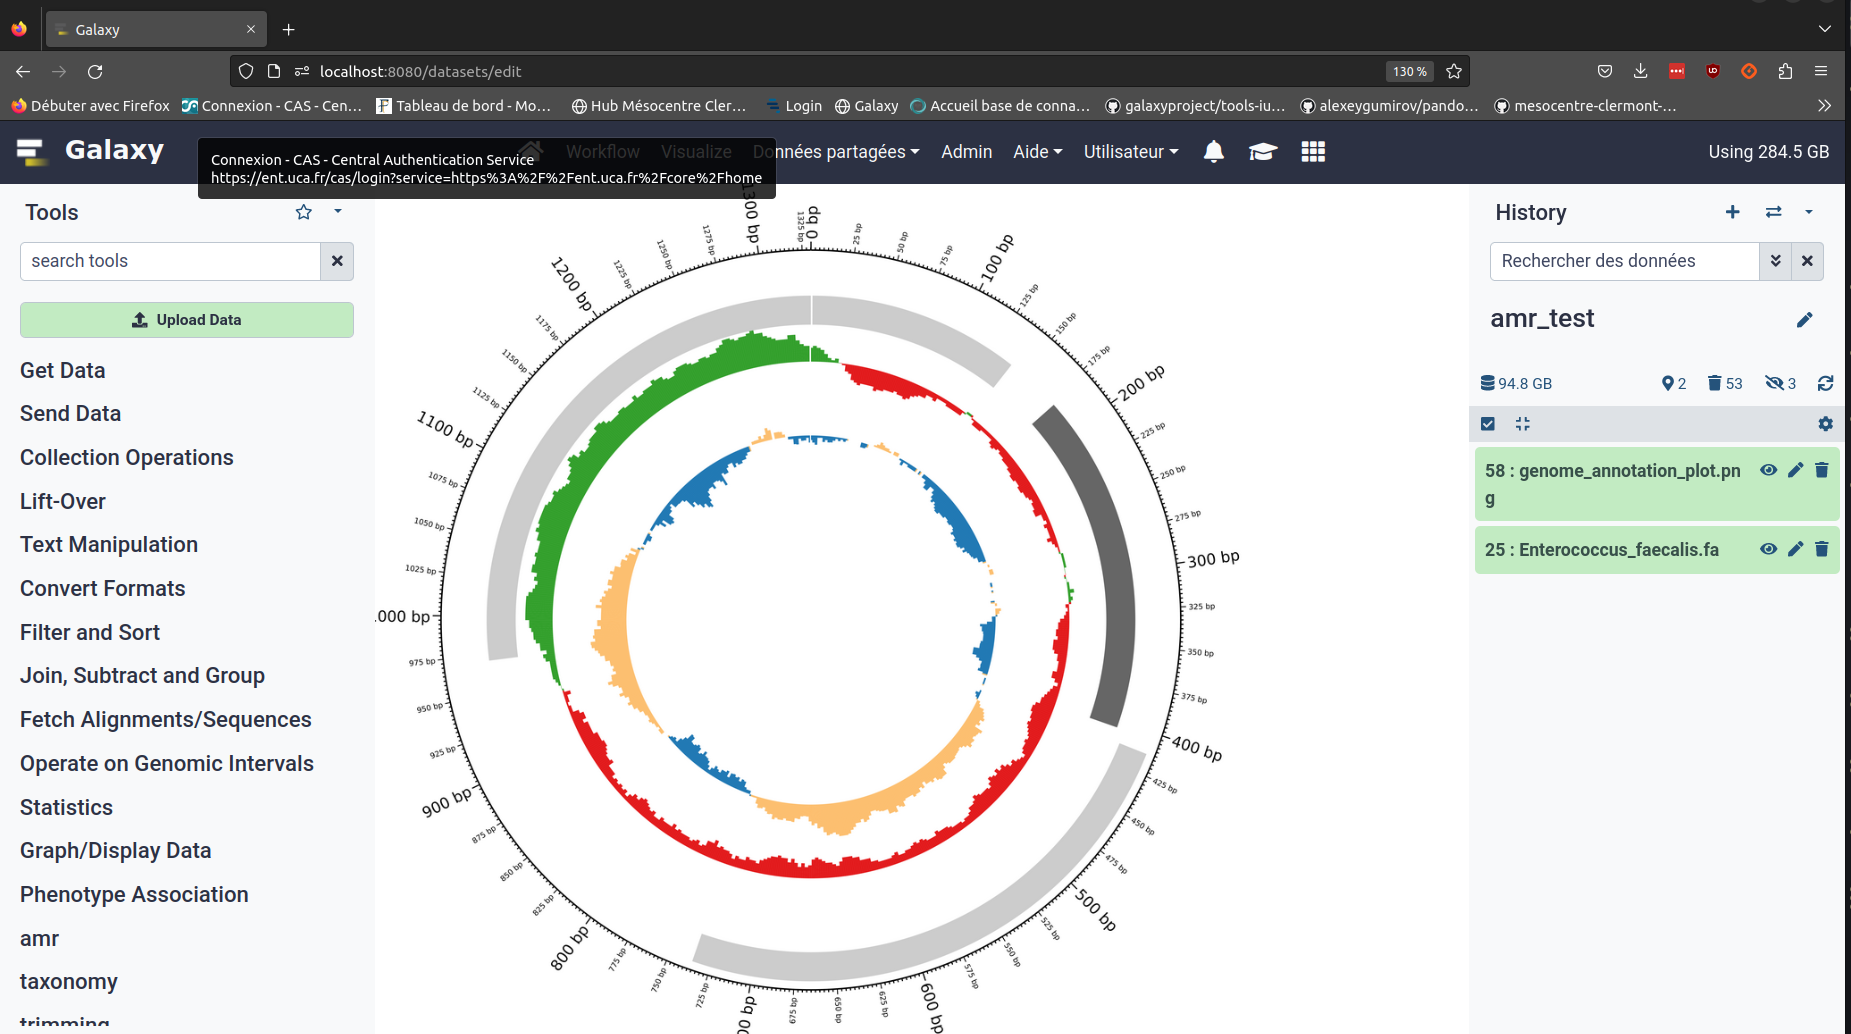
\includegraphics[scale=0.2]{/home/pierre/Seafile/ABROMICS_IFB/projet_aubi/formation_fair/fair_introduction/images/galaxy_screen1.png}}
\only<2>{\centering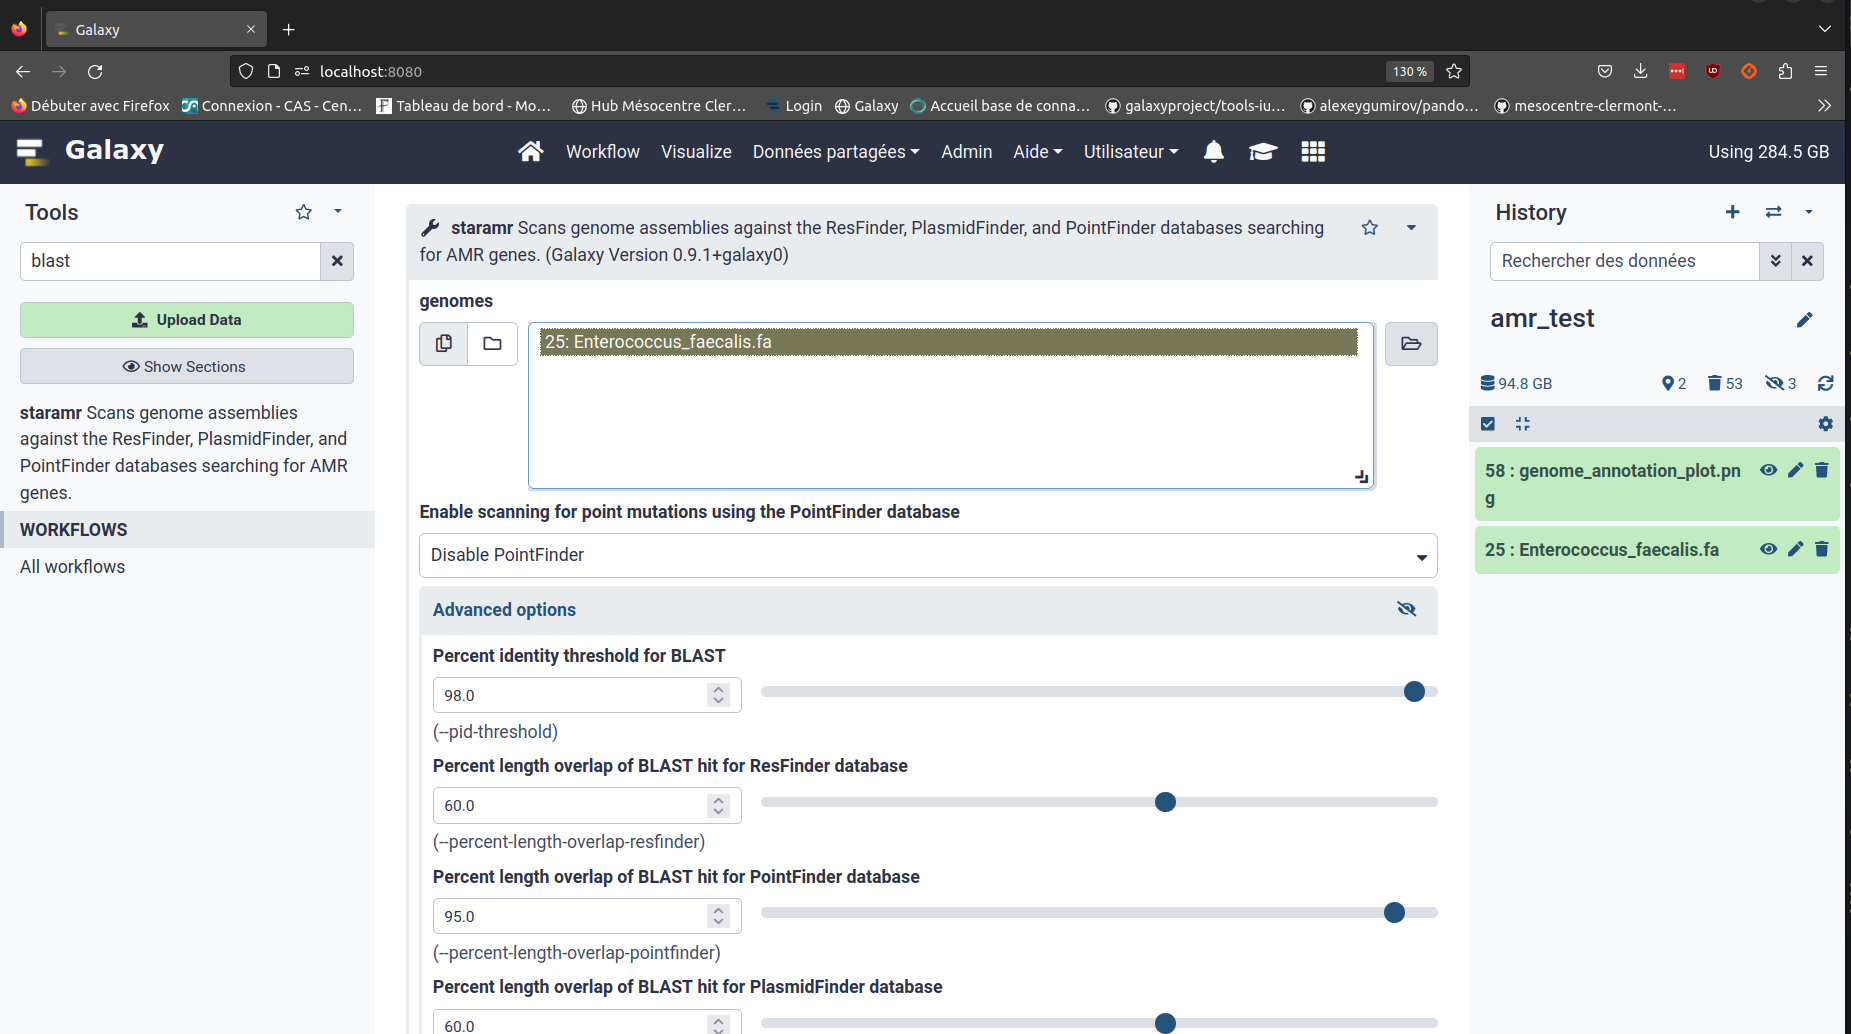
\includegraphics[scale=0.2]{/home/pierre/Seafile/ABROMICS_IFB/projet_aubi/formation_fair/fair_introduction/images/galaxy_screen2.png}}
\only<3>{\centering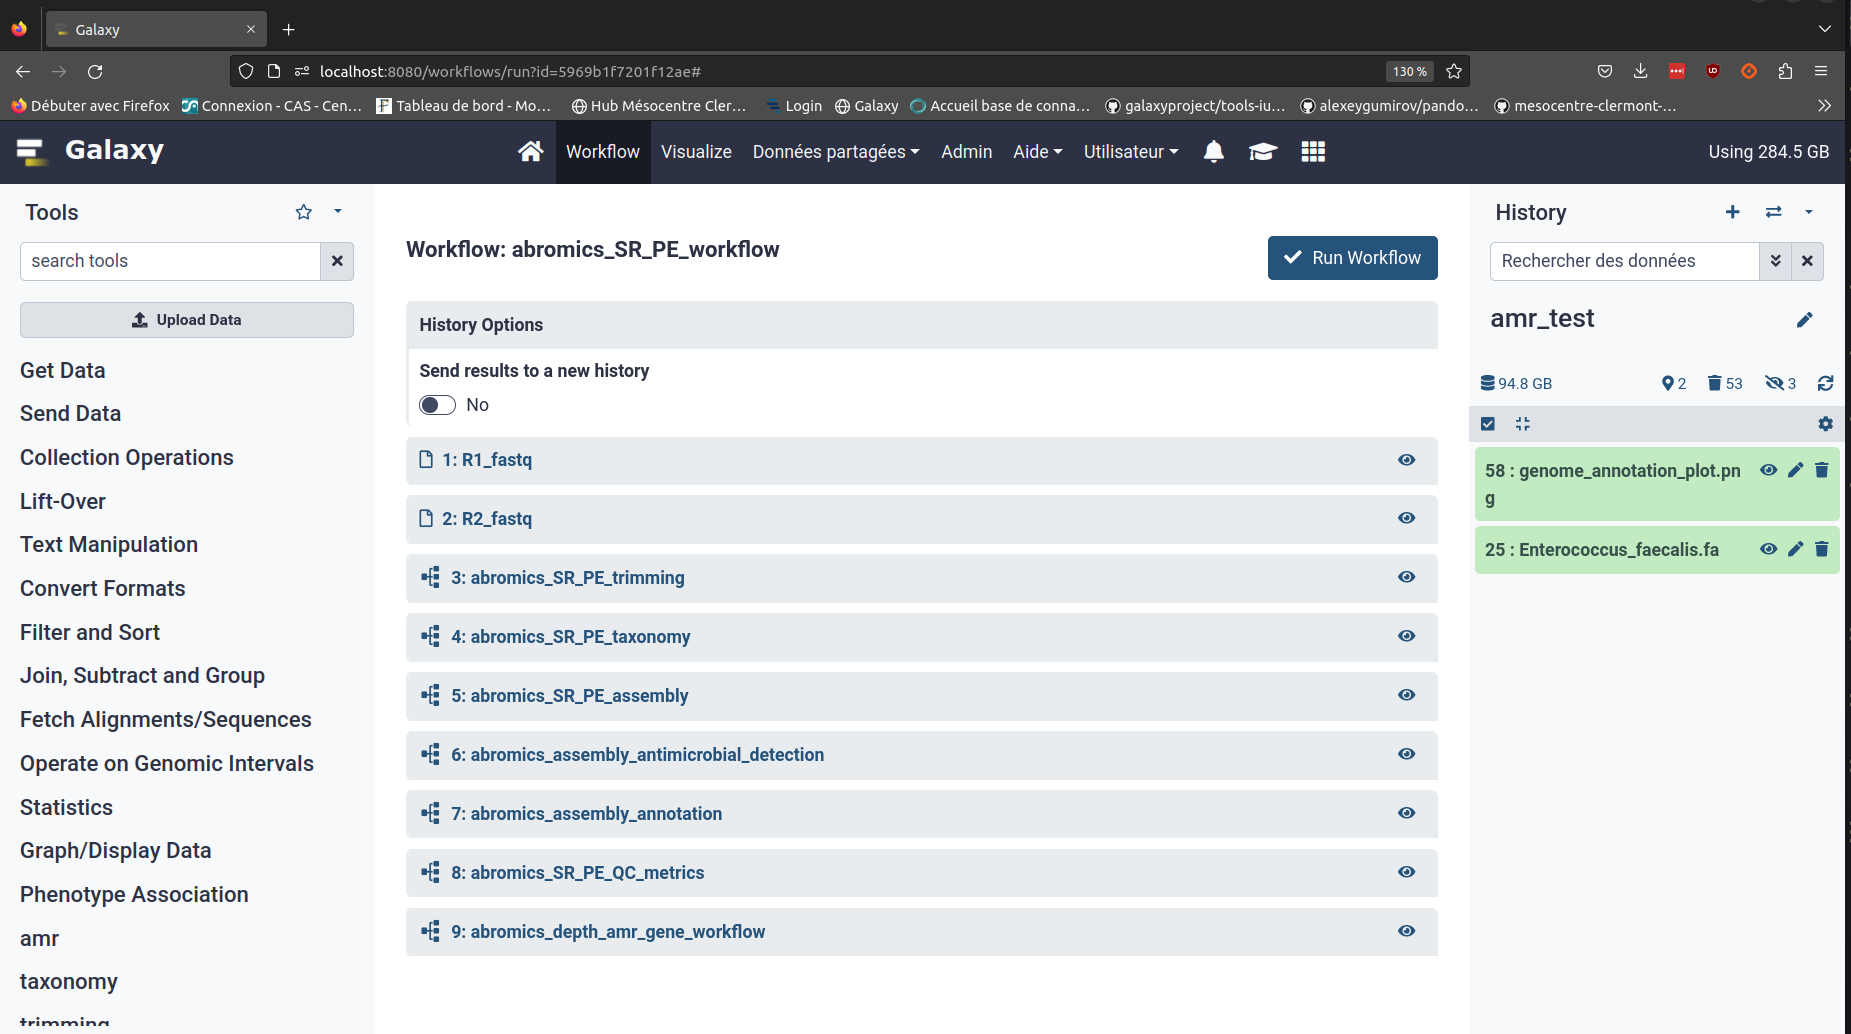
\includegraphics[scale=0.2]{/home/pierre/Seafile/ABROMICS_IFB/projet_aubi/formation_fair/fair_introduction/images/galaxy_screen3.png}}
\only<4>{\centering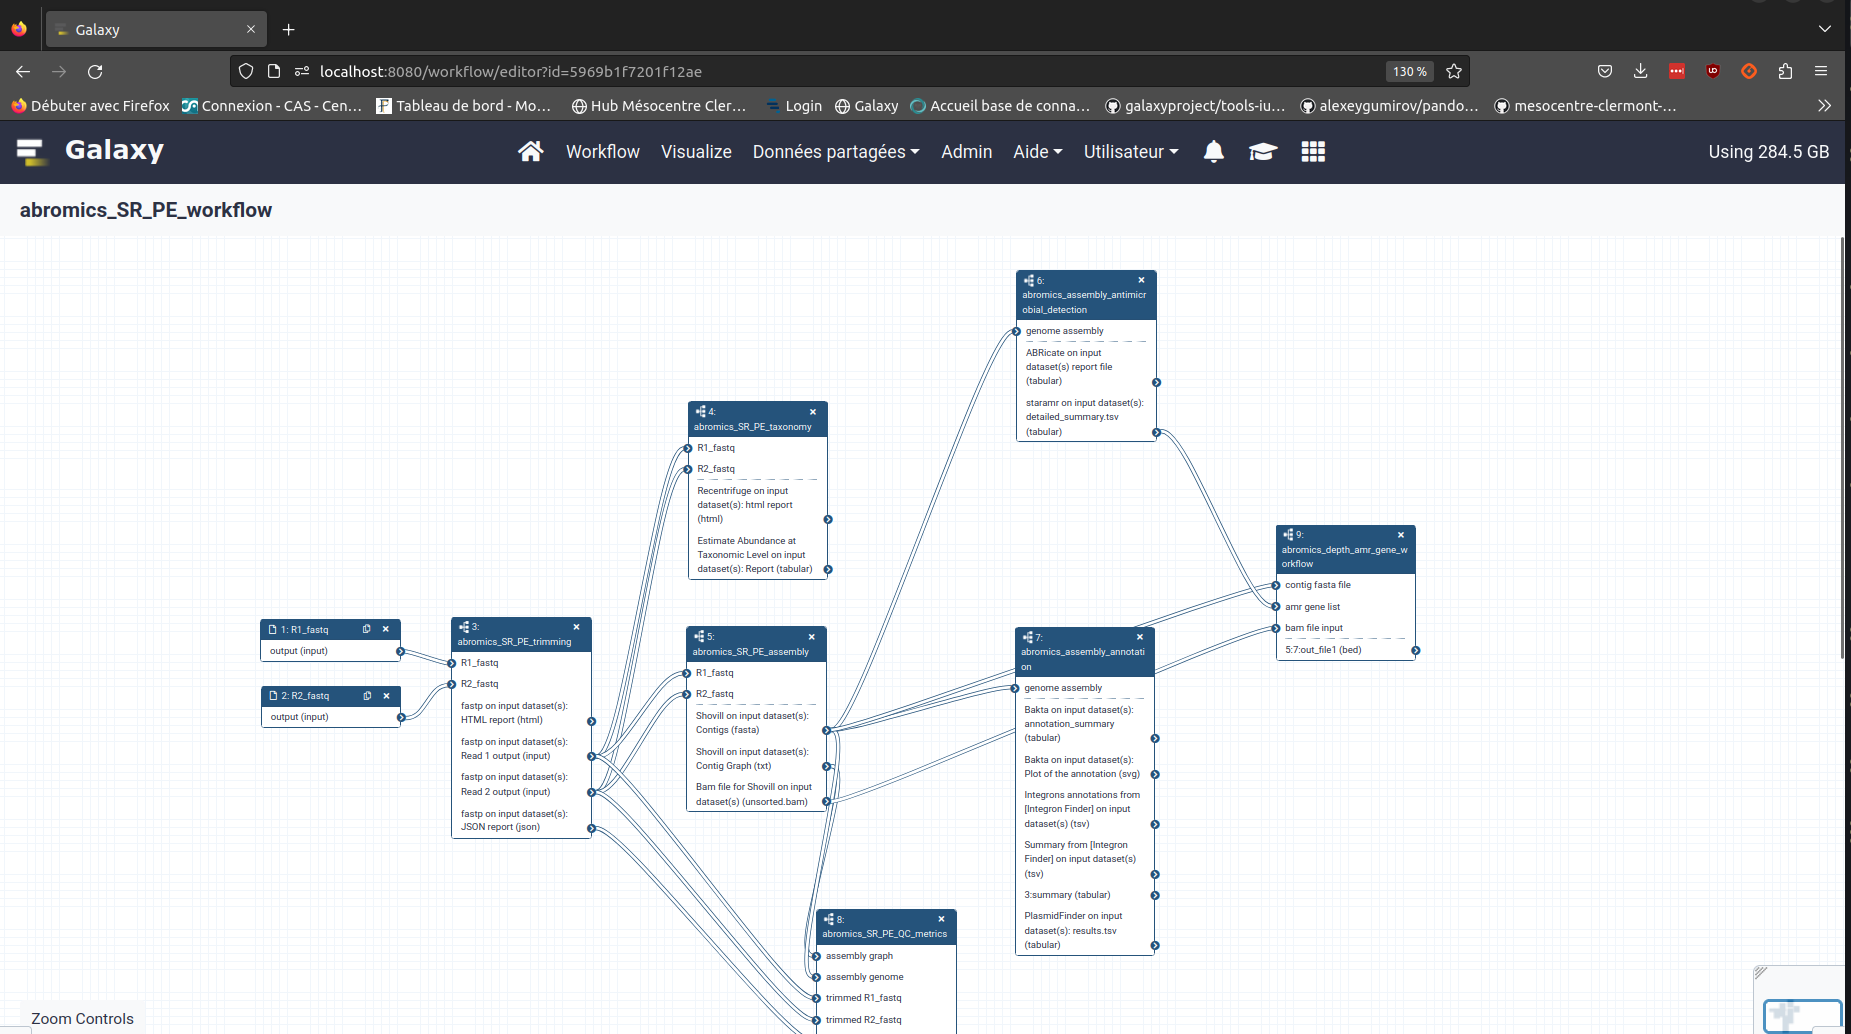
\includegraphics[scale=0.2]{/home/pierre/Seafile/ABROMICS_IFB/projet_aubi/formation_fair/fair_introduction/images/galaxy_screen4.png}}
\end{frame}